\subsection{Overview}
We need to design a system in which the user asks to the system to store an appointment and calculate the best path from a starting location to the appointment location. \\
Since this interaction between user and system can be summarize as:
\begin{enumerate}
	\item User request a service to the system.
	\item System responds to the user with the requested service.
\end{enumerate}
Based on this, we decide to use a client-server architectural approach.
\begin{figure}[H]
	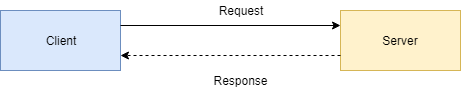
\includegraphics{Img/ClientServerArchitecture}
	\caption{Client Server architecture}
	\label{fig:clientserver}
\end{figure}
Furthermore, the system can be divided into three different subsystems: the presentation layer, the application layer and the data layer as we can see in \autoref{fig:overview}. 
\begin{itemize}
	\item The \emph{Presentation Layer} provides the GUI of the system. This layer contains
	the mobile application and the web pages.
	\item The \emph{Application Layer} contains the logic of the application,that receives the requests from the user, computes the best path to reach the appointment, checks the weather and the road conditions and executes the dynamic web pages of the web site.
	\item The \emph{Data Layer} stores and maintains the data needed from the system to works properly, i.e. user’s information and user’s appointment information.
\end{itemize}
\begin{figure}
	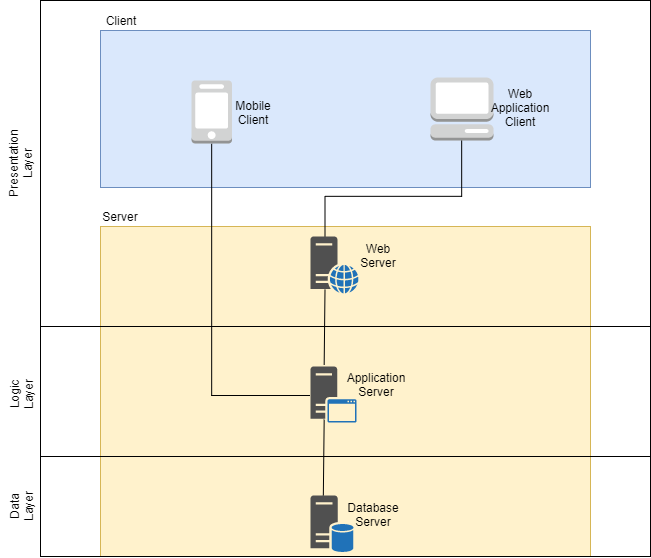
\includegraphics[width=\textwidth, height=\textheight, keepaspectratio=true]{Img/Overview}
	\caption{Overview of the system architecture}
	\label{fig:overview}
\end{figure}

\clearpage


\subsection{Component View}

\subsubsection{Overview}

In \autoref{fig:hlCD} is possible to see the high level components of the system and the interfaces used to connect one to another, where
\begin{itemize}
	\item the \emph{DBMS} provides the database and a way to retrieve data from it;
	\item the \emph{Application Server} provides the main logic of the application;
	\item the \emph{Web Server} provides the static pages and executes the dynamic pages of the web site.
	\item the \emph{Mobile Application} is the mobile application used by a user with his/her smartphone.
	\item the \emph{Web Application} is the application that runs on the user's browser.
\end{itemize}

\begin{figure}
	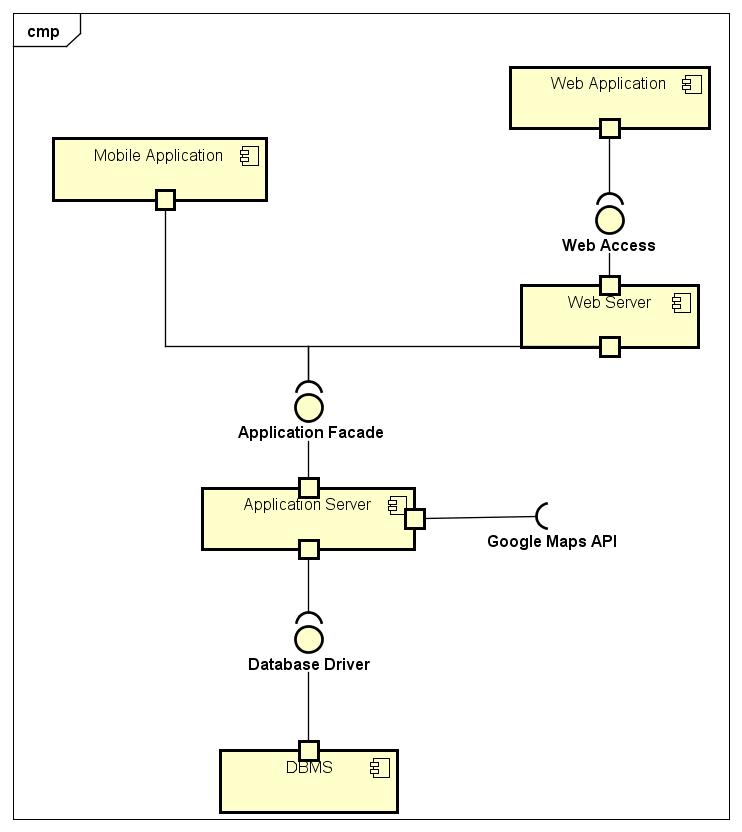
\includegraphics[width = \textwidth, keepaspectratio = true]{Img/HighLevelComponent}
	\caption{High level Component Diagram}
	\label{fig:hlCD}
\end{figure}

\subsubsection{Database View}
The DBMS component provides a database and is DBMS for data storage and their management.
It is possible to access the database only through the Application Server and an appropriate secure interface.
For security and privacy reasons, data are encrypted inside the database.
The Entity-Relationship diagram of the database is showed in \autoref{fig:ERDiagram}.

\begin{figure}
	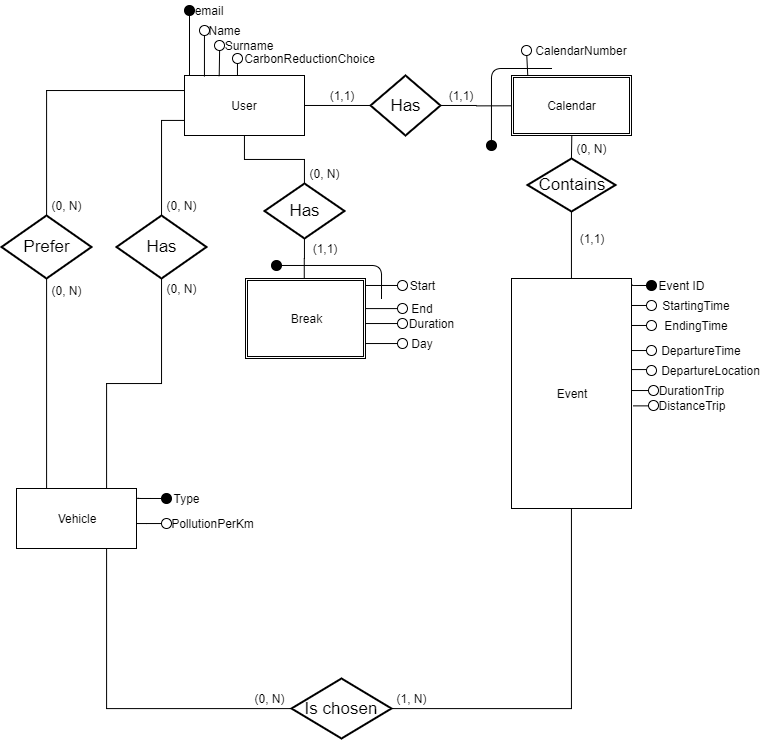
\includegraphics[width = \textwidth, keepaspectratio = true]{Img/ERDiagram}
	\caption{\emph{Entity-Relationship Diagram} of the database}
	\label{fig:ERDiagram}
\end{figure}

\subsubsection{Application Server View}
The \emph{Application Server} contains the main logic of the application. It receives the user's request and interacts with the database to store and retrieves data. 
The \emph{Application Server} as we can see in \autoref{fig:applicationservercomponentCD} is composed of:

\begin{itemize}
	\item \textbf{Authentication Manager}, it manages the request of a user to register or to login into the service. It can access to \emph{Account Data Manager} to retrieves user's information from the database.
	\item \textbf{Profile Manager}, it manages the request of a user to update his/her profile. It can access the \emph{Account Data Manager} in order to retrieves information in the database.
	\item \textbf{Account Data Manager}, it can access all the information about the user's account in the database. 
	\item \textbf{Appointment Manager}, provides to the user the functionalities of creation / modification of appointments. It uses the \emph{Path Calculator} to obtain the best path for the appointment and the \emph{Appointment Data Manager} to stores and retrieves information.
	\item \textbf{Path Calculator}, it is responsible to compute the best path from the starting location defined by the user and the appointment location. To do so, it can access the \emph{Additional Info Facade} to retrieves the user preferences, the weather and road informations. It needs also the \emph{Google Maps API} to retrieves distance and time informations.
	\item \textbf{Weather Information Manager}, it manages weather information retrieving it from an external system via its API, showed in the diagram as \emph{Weather API}.
		\item \textbf{Road Information Manager}, it manages road information retrieving it from an external system via its API, showed in the diagram as \emph{Road API}.
	\item \textbf{Additional Info Facade}, it is a component that implements the \emph{Facade Pattern}, in this way it is possible to reduce the coupling between the \emph{Path Calculator} and the other interfaces from that needs to get information required.
	\item \textbf{Travlendar+ Facade}, it is a component that implements the \emph{Facade Pattern} and provides a common interface for both the \emph{Mobile Application} and the \emph{Web Server}.	
\end{itemize}

\begin{figure}
	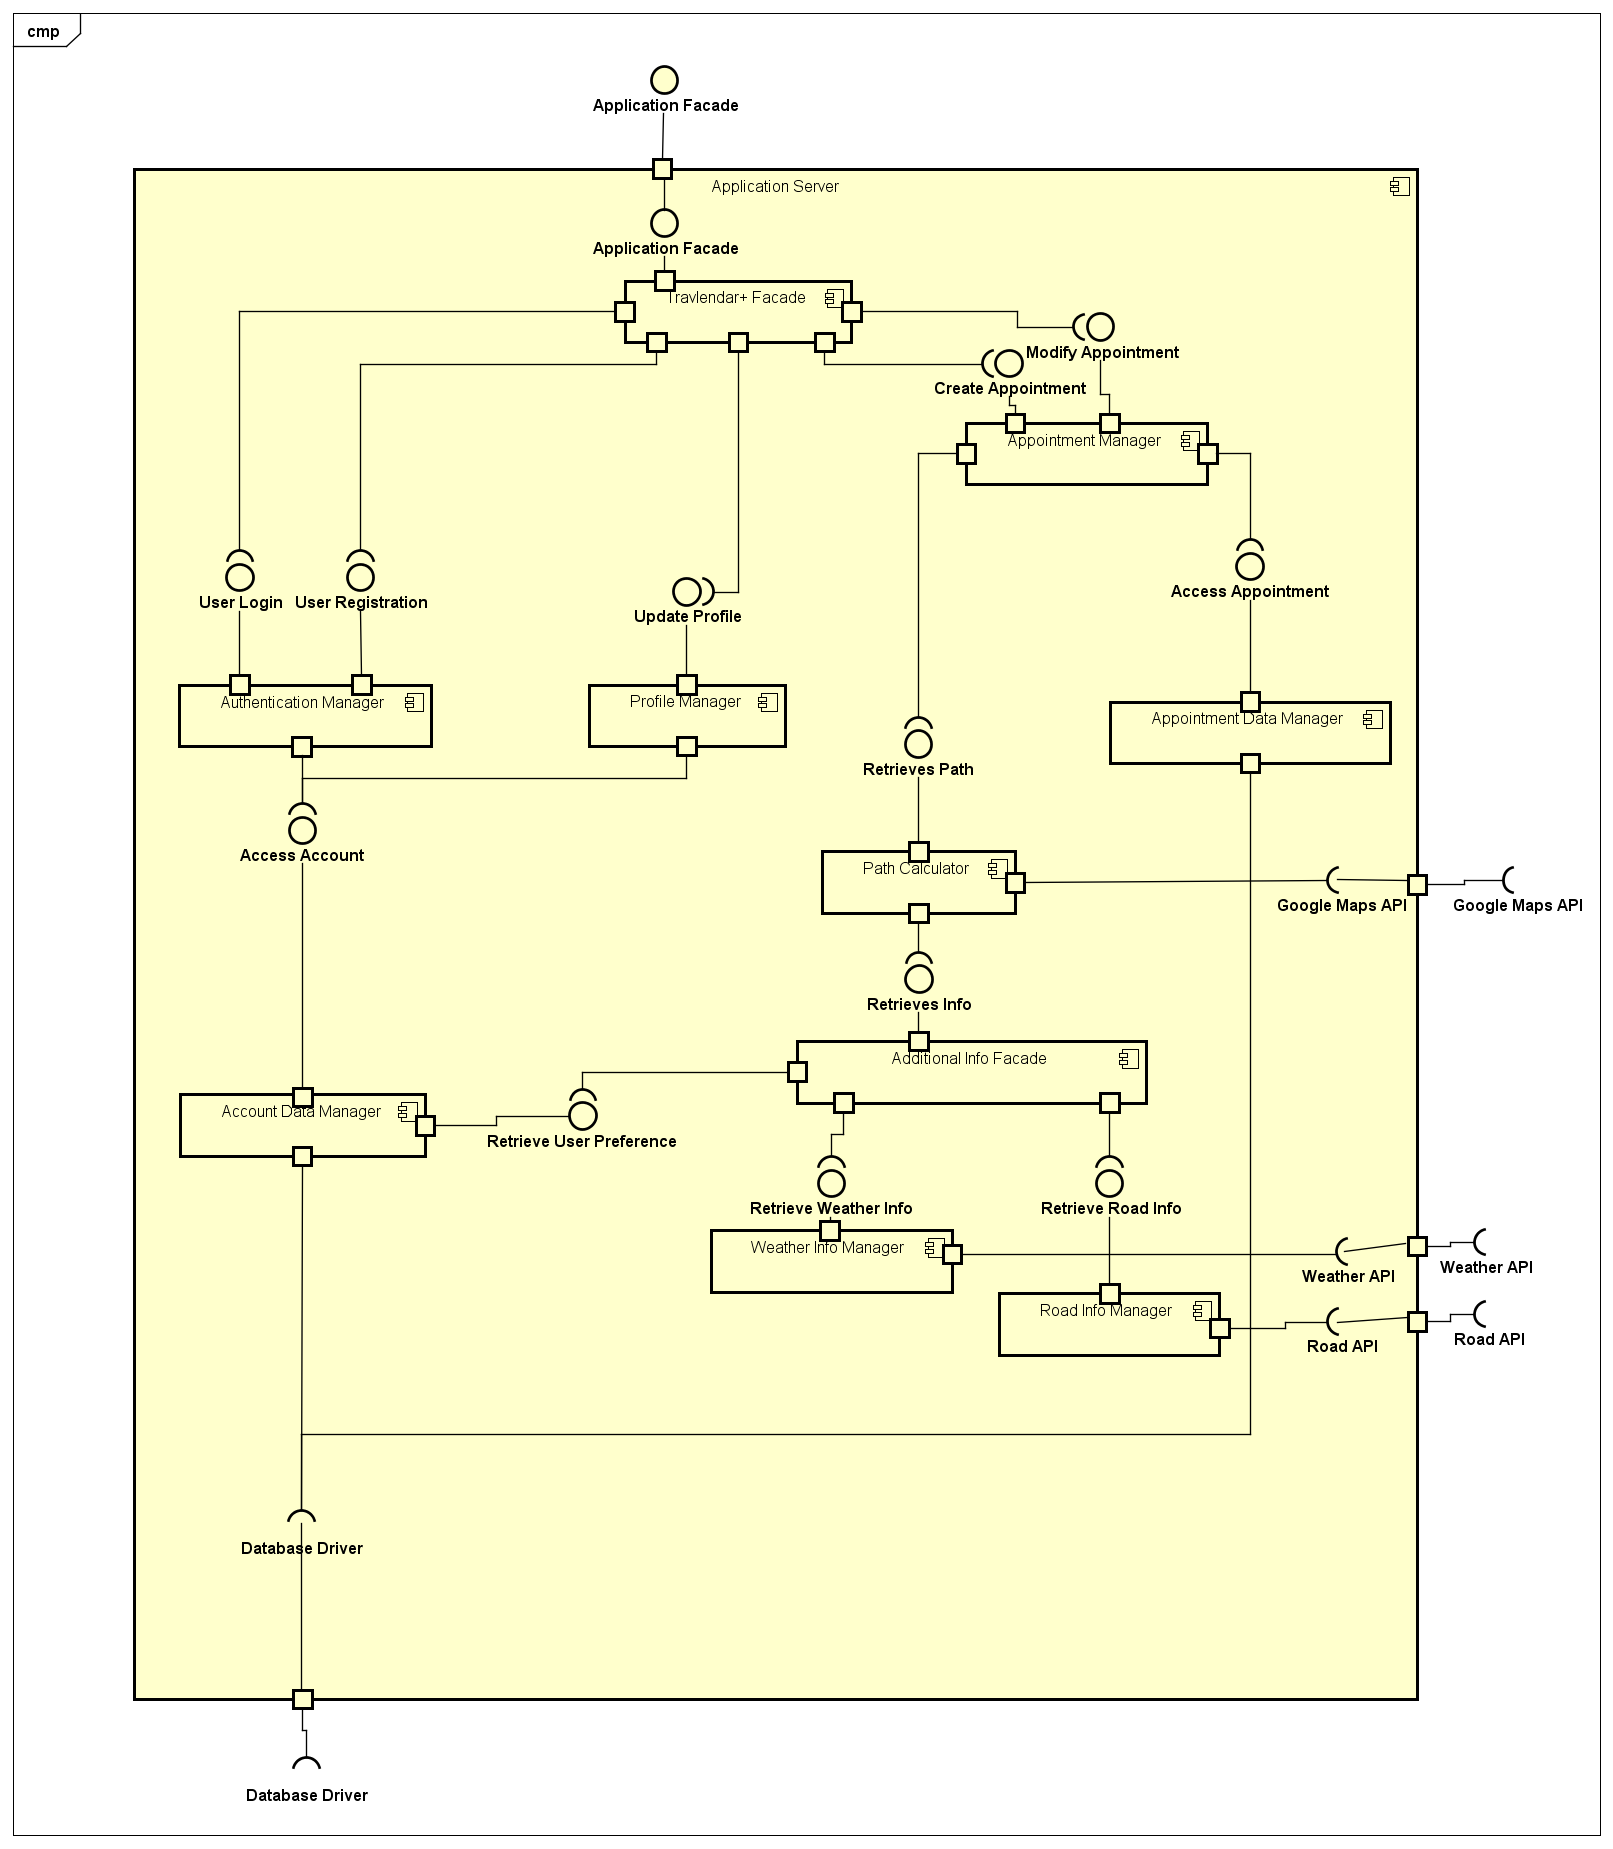
\includegraphics[width = \textwidth, height = \textheight, keepaspectratio = true]{Img/ApplicationServerCD}
	\caption{\emph{Application Server} component diagram}
	\label{fig:applicationservercomponentCD}
\end{figure}

\subsubsection{Web Server}
Since the presence of a \emph{Web Application}, it is necessary a dedicated \emph{Web Server} responsible to executes the web site’s dynamic pages and provides the static pages to the user’s browser.
The \emph{Web Server} interacts with the \emph{Application Server} to get the proper information to fill up the pages.
The \emph{Web Server} also sends data from the user’s browser to the \emph{Application Server} to store inside the database.

\subsubsection{Mobile Application}
The \emph{Mobile Application} is used by the user via its own smart device. The \emph{Mobile Application} communicates directly the \emph{application server} with a dedicated communication protocol.
The component diagram of the \emph{Mobile Application} is showed in \autoref{fig:mobileapplicationCD}.
The description of the components is the follow:
\begin{itemize}
	\item \textbf{User View} is responsible of the graphical representation of the app and the interactions with the user.
	\item \textbf{GPS Manager} is responsible to interact with the GPS Module of the smart device.
	\item \textbf{DBMS}, is a physical view of the main database while storing only the current user's data. 
	\item \textbf{Controller}, is responsible to interact with the \emph{Application Server} and link together the other components.
\end{itemize}

\begin{figure}
	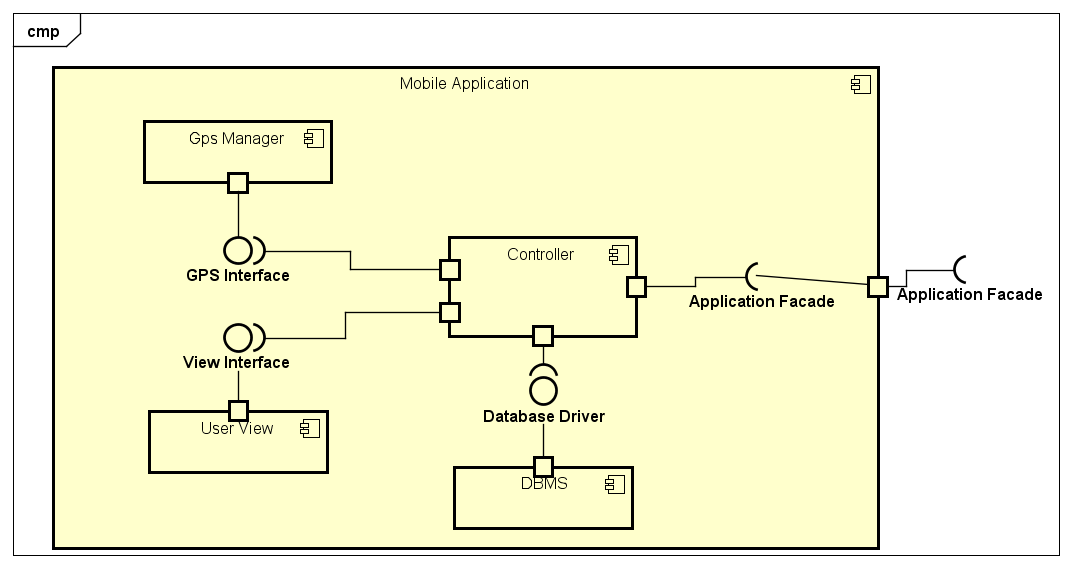
\includegraphics[width = \textwidth, keepaspectratio = true]{Img/MobileApplication}
	\caption{\emph{Mobile Application} component diagram}
	\label{fig:mobileapplicationCD}
\end{figure}

\clearpage
\subsection{Deployment View}

\clearpage
\subsection{Runtime View}

\clearpage
\subsection{Component Interfaces}

\clearpage
\subsection{Selected architectural styles and patterns}

\clearpage
\subsection{Other design decision}